%!TEX encoding = UTF-8 Unicode

\documentclass{article}

\usepackage{geometry}
\geometry{top=3cm,bottom=3cm}
\usepackage{graphicx}
\usepackage[colorlinks,linkcolor=red]{hyperref}
\usepackage{CJKutf8} %调用 xeCJK 宏包
    %\setCJKmainfont{SimSun}

\begin{CJK}{UTF8}{}
\renewcommand{\figurename}{图}
\title{Aggregated Residual Transformations for Deep Neural Networks}
\date{}
\begin{document}
\maketitle
\begin{center}
\fontsize{14pt}{14pt}\href{https://arxiv.org/pdf/1611.05431.pdf}{论文链接}
\end{center}
\section{概述}

\paragraph{} 
本文是对于深度学习网络的进一步探索,文中作者提出了一种改进版的ResNet网络框架,名为ResNext。相对于但当年的ResNet网络的将网络变深的思想,ResNext借鉴了Inception网络架构的思想,尝试将网络拓宽,在保留餐叉结构的情况下,引入“cardinality”的概念,将网络拓宽,在imagenet与coco数据集上具有不错的性能表现。
\section{主要架构}
\paragraph{}
作者提出的ResNext网络结构可以看做是ResNet的改进版。如图1,传统的残差结构可以表示为:$g(x)=x+f(x)$, 其中$g(\cdot)$表示残差结构的输出,$f(\cdot)$表示残差结构内部的卷积、激活函数、batch normalization等操作。
\begin{figure}[ht]
\centering
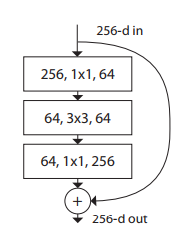
\includegraphics[scale=0.8]{figure1.png}
\caption{残差结构图}
\label{fig:label}
\end{figure}
\paragraph{}
对于ResNet来说,增强网络性能最主要也是最常用的方法是增加网络的深度,即增大网络的层数,在一定范围内,增大网络层数的确会带来性能的提升,随着网络层数的增加,带来的性能提升也会逐渐减小,但是网络层数增加所带来的计算量的增加却是难以回避的问题,同时网络层数的增加也会带来收敛困难的问题,再此基础上作者借鉴了inception的结构,如图2所示。inception在图像分类等许多计算机视觉任务上表现出了很强大的性能,但是inception的结构偏向于复杂,所以作者改进的ResNet网络,提出了ResNext结构。
\begin{figure}[ht]
\centering
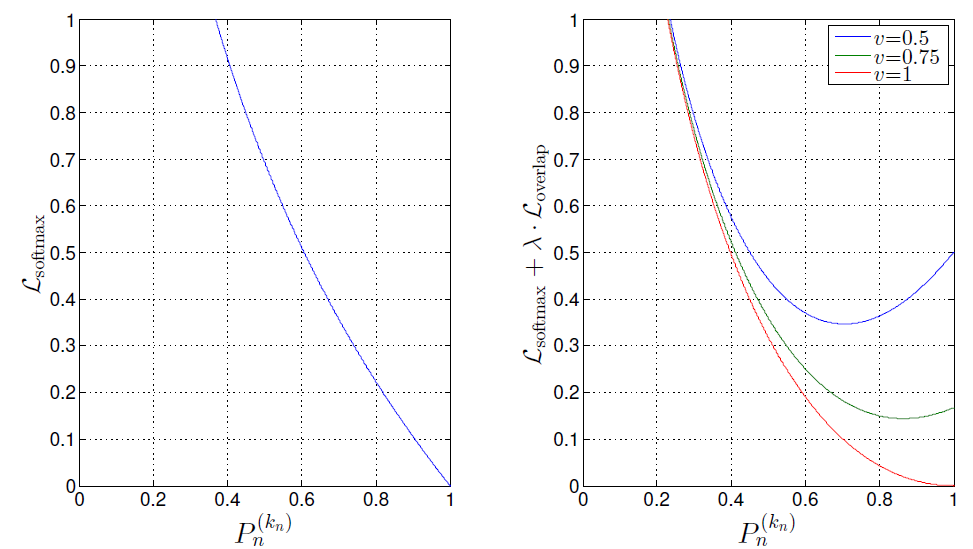
\includegraphics[scale=0.6]{figure2.png}
\caption{残差结构图}
\label{fig:label}
\end{figure}
\paragraph{}
ResNext结构与ResNet架构十分相似,只是在内部结构上做了改进,如图3,将卷积结构进行扩张,原本一个卷积操作变成了多个并行。这样的操作在没有带来更多计算量的情况下,极大地提升网络的性能。原本残差结构152层网络才能达到的性能,使用ResNext结构只需要101层。
\begin{figure}[ht]
\centering
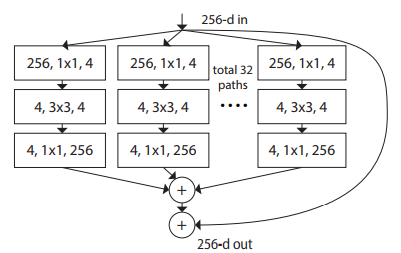
\includegraphics[scale=1]{figure3.png}
\caption{残差结构图}
\label{fig:label}
\end{figure}
\section{总结}
\paragraph{}
ResNext网络极大提升网络性能,但是带来的计算量增加几乎可以忽略不计,同时该网络可以很好的作为其他视觉任务的基础网络。美中不足的是该网络在mxnet框架上耗时严重,问题应该是出在ResNext使用group的方式实现。在mxnet中split操作很耗时间,期待后续版本升级能解决此问题。

\end{CJK}
\end{document}
